\documentclass[letterpaper]{article}

%%%%%%%%%%%%%%%%%%%%%%%%%%%%%%%%%%%%%%%%%%%%%%%%%
%%%%                  HI!                    %%%%
%%%%        THIS IS THE SSI-BIOLOGY			 %%%%
%%%%      GENERIC PROCEDURE TEMPLATE :) 	 %%%%
%%%%      IT MIGHT LOOK SCARY, BUT IT'S 	 %%%%
%%%%           PRETTY EASY TO USE 			 %%%%
%%%%%%%%%%%%%%%%%%%%%%%%%%%%%%%%%%%%%%%%%%%%%%%%%

%%%%%%%%%%%%%%%%%%%%%%%%%%%%%%%%%%%%%%%%%%%%%%%%%%%%%%%%%%
%%%%      RIGHT NOW YOU'RE LOOKING AT BOILERPLATE     %%%%
%%%%  THAT IS, THINGS YOU DON'T HAVE TO CHANGE (EVER) %%%%
%%%%     SCROLL DOWN FOR THE THINGS YOU SHOULD PAY    %%%%
%%%%    ATTENTION TO :)  (YOU'LL KNOW WHEN TO STOP)   %%%%
%%%%%%%%%%%%%%%%%%%%%%%%%%%%%%%%%%%%%%%%%%%%%%%%%%%%%%%%%%


%% Language and font encodings
\usepackage[english]{babel}
\usepackage[utf8x]{inputenc}
\usepackage[T1]{fontenc}

%% Sets page size, footer, indent and margins
\usepackage[a4paper,top=2.5cm,bottom=2cm,left=2.25cm,right=2.25cm,marginparwidth=2.25cm]{geometry}
\setlength\parindent{0pt}
\setlength{\footskip}{55pt}

%% Useful packages
\usepackage{amsmath}
\usepackage{graphicx}
\usepackage{fancyhdr}
\pagestyle{fancy}
\usepackage{textcomp}
\usepackage{gensymb}
\usepackage{hyperref}
\usepackage{readarray}
\usepackage{verbatimbox}
\usepackage{framed}
\usepackage[dvipsnames]{xcolor}
\usepackage{tcolorbox}
\usepackage{colortbl}
\usepackage{libertine} 
\usepackage{siunitx}


% Safety Environment 
\definecolor{safetyFrame}{HTML}{FFFFFF}
\newenvironment{safety}{%
\begin{tcolorbox}[width=\textwidth, colframe=safetyFrame, arc=1.5mm]
}%
{\end{tcolorbox}}


% Footer
\lfoot{
\includegraphics[height=1.5cm]{1000x350-Horiz-Logo-WhiteRed-BlackText.png}}

% Substitution Commands
\newcommand{\tdt}{Terminal Deoxynucleotidyl Transferase}
\newcommand{\C}{\degree{}C}
\newcommand{\uL}{\micro{}L}
\newcommand{\BdATP}{3'-O-(2-nitrobenzyl)-2'-dATP}

%Custom Commands
\newcommand{\B}[1]{\textbf{#1}}

% Safety Info
\newcommand{\SYBRGOLD}{\item{\B{SYBR Gold} has no data available addressing the mutagenicity or toxicity of SYBR® Gold nucleic acid gel stain. Because this reagent binds to nucleic acids, it should be treated as a potential mutagen and handled with appropriate care. The DMSO stock solution should be handled with particular caution as DMSO is known to facilitate the entry of organic molecules into tissues.\cite{sybrGold}}}
\newcommand{\SYBRI}{\item{\B{SYBR Green I} is a mutagen and can penetrate laboratory gloves in a relatively short period of time, please change your gloves in the event of contamination. See \url{http://www.sigmaaldrich.com/MSDS/MSDS/DisplayMSDSPage.do?country=US&language=en&productNumber=S9430&brand=SIAL} for more information on the specifics of SYBR Green I. 
}}
\newcommand{\ETBR}{\item{\B{Ethidium Bromide} is a \B{serious mutagen} and is \B{significantly carcinogenic}. If working with considerable amounts, a \B{fume hood and respirator} are warranted. For more information see \url{https://www.sciencelab.com/msds.php?msdsId=9927667}
}}


% Shortcuts

%Stop Point (Optional)
\newcommand{\stopPoint}{\begin{center}
\rule{0.5\textwidth}{.4pt}\\
\vspace{1mm} 
OPTIONAL STOP POINT\\
\rule{0.5\textwidth}{.4pt}
\end{center}}

\newcommand{\RstopPoint}{\begin{center}
\rule{0.5\textwidth}{.4pt}\\
\vspace{1mm} 
RECOMMENEDED STOP POINT\\
\rule{0.5\textwidth}{.4pt}
\end{center}}

% Dilution Macro
\newcommand{\Dilution}[4]{
\subsection{#2}
\begin{enumerate}
\item{Vortex #2 stock}
\item{Pipette #1\uL{} #2 into a PCR Tube}
\item{Pipette #3\uL{} #4 into solution}
\item{Vortex until mixed}
%\item{Pipette $#2\mu L$ Water into solution}
\end{enumerate}
}

% Gel Macro
\newcommand{\gel}[4]{
\begin{figure}[ht]
\label{#2}
\begin{center}
\includegraphics[width=0.45\textwidth]{#1}
\caption{#2}
\end{center}
\subsection{#3 Analysis}
#4
\end{figure}
}

% Well plate Macro
\newcommand{\wellplate}[2]{
\getargsC{#1}
\begin{tabular}{*{1}{>{\columncolor{blue!20}}l}|l|l|l|l|l|l|l|l|l|l|l|l|}
\rowcolor{blue!20}%
 & 1  & 2  & 3  & 4  & 5  & 6 & 7 & 8 & 9 & 10 & 11 & 12\\ \hline
\ifdefined\argxii
A & \argi & \argii & \argiii & \argiv & \argv & \argvi & \argvii & \argviii & \argix & \argx & \argxi & \argxii \\ \hline\fi
\ifdefined\argxxiv
B & \argxiii & \argxiv & \argxv & \argxvi & \argxvii & \argxviii & \argxix & \argxx & \argxxi & \argxxii & \argxxiii & \argxxiv \\ \hline\fi
\ifdefined\argxxxvi
C & \argxxv & \argxxvi & \argxxvii & \argxxviii & \argxxix & \argxxx & \argxxxi & \argxxxii & \argxxxiii & \argxxxiv & \argxxxv & \argxxxvi \\ \hline\fi
\ifdefined\argxlviii
D & \argxxxvii & \argxxxviii & \argxxxix & \argxl & \argxli & \argxlii & \argxliii & \argxliv & \argxlv & \argxlvi & \argxlvii & \argxlviii \\ \hline\fi
\ifdefined\arglx
E & \argxlix & \argl & \argli & \arglii & \argliii & \argliv & \arglv & \arglvi & \arglvii & \arglviii & \arglix & \arglx \\ \hline\fi
\ifdefined\arglxxii
F & \arglxi & \arglxii & \arglxiii & \arglxiv & \arglxv & \arglxvi & \arglxvii & \arglxviii & \arglxix & \arglxx & \arglxxi & \arglxxii \\ \hline\fi
\ifdefined\arglxxxiv
G & \arglxxiii & \arglxxiv & \arglxxv & \arglxxvi & \arglxxvii & \arglxxviii & \arglxxix & \arglxxx & \arglxxxi & \arglxxxii & \arglxxxiii & \arglxxxiv \\ \hline\fi
\ifdefined\argxcvi
H & \arglxxxv & \arglxxxvi & \arglxxxvii & \arglxxxviii & \arglxxxix & \argxc & \argxci & \argxcii & \argxciii & \argxciv & \argxcv & \argxcvi \\ \hline\fi
\end{tabular}
}

\newcommand{\tdtSafety}{\item{\textbf{\tdt{}} is toxic if inhaled. May cause cancer. Toxic to aquatic life with long lasting effects. Avoid breathing dust/fume/gas/mist/vapours/spray. Use personal protective equipment as required. If Inhaled: Remove victim to fresh air and keep at rest in a position comfortable for breathing. Dispose of contents/container in accordance with local/regional/national/international regulations.\cite{Invitrogen2002}}}

%%%%%%%%%%%%%%%%%%%%%%%%%%%%%%%%%%%%%%%%%%%%%%%
%%%%%%%%%%%%%%%%%%%%%%%%%%%%%%%%%%%%%%%%%%%%%%%
%%%%%%%%%%%%% End of Boiler Plate %%%%%%%%%%%%%
%%%%%%%%%%%%%%%%%%%%%%%%%%%%%%%%%%%%%%%%%%%%%%%
%%%%%%%%%%%%%%%%%%%%%%%%%%%%%%%%%%%%%%%%%%%%%%%

%%%%%%%%%%%%%%%%%%%%%%%%%%%%%%%%%%%%%%%%%%%%%%%
%%%%%   AKA YOU WRITE AFTER THIS POINT    %%%%%
%%%%%%%%%%%%%%%%%%%%%%%%%%%%%%%%%%%%%%%%%%%%%%%


\title{\BdATP{} Incorporation Detection with PAGE Assisted Precision} % CHANGE THIS
\author{Written by \textbf{Michael Uttmark}\\ % CHANGE THIS 
		Not Peer Reviewed\\%Checked by \textbf{}\\ % CHANGE THIS
        For the Stanford Student Space Initiative Biology Subteam}

\begin{document}

\maketitle
\section{Procedure Purpose} % CHANGE THIS
Determine if the the modified nucleotide, \BdATP{}, can be noticeably incorporated by \tdt{} in "standard conditions" while determining the blocking efficacy \& purity of our \BdATP{} stock.
\begin{figure}[ht]
\centering
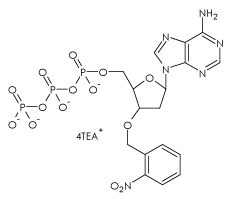
\includegraphics[width=2in]{1.png}
\caption{\BdATP{}}
\label{bdatp}
\end{figure}
\section{Overview} % CHANGE THIS 
This lab will attempt to append \BdATP{} to a \textbf{very short (5bp) primer}. The effectiveness of this attempt will be determined by attempting to form a homopolymer on the modified primer. If a homopolymer is formed, the blocking groups did not effectively prevent their formation. This could be due to many reasons (the most likely of which being that the blocking groups either (1) were appended without the 2' nitrobenzyl due to sample degradation or (2) were not appended). If the homopolymer was not formed (but a homopolymer was formed on the controls) it follows that the blocking groups prevented the formation of the homopolymer, likely due to them preforming their intended function. Moreover, all samples will be run on a PAGE gel in order to achieve single nucleotide resolution. This will allow us to confirm that the \BdATP{} is the only base appended to the "blocked" sample. A ddATP control will help as well.

% Safety First! ALSO, % CHANGE THIS
\section{Safety Information}
\begin{safety}
\begin{enumerate}
\SYBRGOLD{} % For select reagents, I've created custom commands so we don't have to copy and paste every time :)
\tdtSafety{}
\item{Working in a communal lab space is dangerous. Do not assume your fellow workers cleaned up sufficiently}
\end{enumerate}
\end{safety}

\section{Materials}
\begin{itemize}
\item{Primer: ATGGACATGCCCCTACTTGCATAAG}
\item{100mM \BdATP{} Stock}
\item{100mM dNTP Stock}
\item{100mM dATP Stock}
\item{100mM ddATP Stock}
\item{5X \tdt{} Buffer}
\item{\tdt{} Stock (20U/\uL{})}
\item{Nuclease Free Water}
\item{TBE Buffer}
\item{15\% Urea Denaturing Gels}
\item{SYBR Gold}
\end{itemize}
% Now for the _good_ stuff  
\section{Procedure}% CHANGE THIS
\begin{enumerate} 
\subsection{Sample Preparation}
\item{Remove \BdATP{}, \tdt{}, primer, \tdt{}  buffer, ddATP stock and dATP stock from -20\C{} freezer}
\item{Let \BdATP{} thaw on ice in dark}
\item{Other reagents can thaw on ice in the light}
\subsection{Attempted blocking}
\item{Label three PCR Tubes A, B and D, respectively}
\item{Pipette 10\uL{} of nuclease free water into both PCR Tubes}
\item{Pipette 4.0\uL{} 5X \tdt{} reaction buffer into both PCR Tubes}
\item{Dilute Nucleotides:
\begin{enumerate}
\item{Label a PCR Tube "dATP Dilute"}
\item{Pipette 9\uL{} of nuclease free water into PCR Tube}
\item{Pipette 1\uL{} of dATP stock into PCR Tube}
\item{Vortex directly before use}
\end{enumerate}
\begin{enumerate}
\item{Label a PCR Tube "dd Dilute"}
\item{Pipette 9\uL{} of nuclease free water into PCR Tube}
\item{Pipette 1\uL{} of ddATP stock into PCR Tube}
\item{Vortex directly before use}
\end{enumerate}
NOTE: This step can be skipped, as this dilute has already been made. The dilution instructions are redundant, and are here in case we want to repeat the experiment in the future.
\begin{enumerate}
\item{Label a PCR Tube "\textbf{BdATP} Dilute" (make this \textit{very} clear)}
\item{Pipette 9\uL{} of nuclease free water into PCR Tube}
\item{Pipette 1\uL{} of \BdATP{} stock into PCR Tube}
\item{Keep in \textbf{dark} and vortex directly before use}
\end{enumerate}
}
\item{Pipette .5\uL{} of primer into all three PCR Tubes}
\item{Pipette 2\uL{} of dATP dilute into PCR Tube A}
\item{Pipette 2\uL{} of \BdATP{} dilute into PCR Tube B}
\item{Pipette 2\uL{} of ddATP dilute into PCR Tube D}
\item{Gently pipette 1.5\uL{} \tdt{} (20 U/\uL{}) into all three PCR Tubes}
\item{Incubate sample at 37\C{} for 30 minutes}\\
Note: \textbf{Do NOT} deactivate \tdt{} 
\stopPoint{} 
\subsection{Extending}
Based off of our standard \tdt{} extending procedure \cite{genTdT}.
\item{Label two PCR Tubes C and X, respectively}
\item{Pipette 10\uL{} nuclease free water into PCR Tube C (see above, \textbf{ATTEMPTED BLOCKING})}
\item{Pipette 10\uL{} of nuclease free water into PCR Tube X (see above, \textbf{CONTROLS})}
\item{Pipette .5\uL{} of primer into both PCR Tubes}
\item{Set PCR Tube X aside.}
\item{Pipette 4.0\uL{} 5X \tdt{} reaction buffer into PCR Tube C}
\item{Pipette .6\uL{} of dNTP stock into PCR Tube \textbf{C}}
\item{Pipette .4\uL{} of dNTP stock into PCR Tubes \textbf{A, B}}
\item{Gently pipette 1.5\uL{} \tdt{} (20 U/\uL{}) into \textbf{PCR Tube C} (note, this is not from the standard 15U\uL{} stock)}
\item{Incubate \textbf{all} samples at 37\C{} for 30 minutes}\\
\RstopPoint{} 
\subsection{Analysis}



\subsubsection{Prepare Gel}
\item{Prepare a 15\% Denaturing Urea-PAGE gel. Rinse each well with 15 uL of .5X TBE buffer. Allow to pre-run at 200V for 20 minutes prior to continuing.}

\subsubsection{Run Gel}
NOTE: Ensure that the loading dye has Bromophenol Blue in it.
\item{Add 8\uL of samples A, B, D, C and X with 1.5\uL{} of loading dye for a total volume of 8\uL to gel respectively, left to right with the wells at the top.}
\item{Add 10\uL{} of Loading Dye to the well twice to the right of X (the seventh well from the left).}
\item{Add an appropriate amount of ladder (annotate the amount added on this sheet) the the far right well (wells at the top).}
\item{Add a 50/50 combination of sample \textbf{B} and sample \textbf{C} to the sixth well. That is, add \textbf{3\uL{}} of sample \textbf{B}, \textbf{3\uL{}} of sample \textbf{B} and \textbf{1.2}\uL{} of loading dye to the sixth well, from the left with the wells at the top.}
\item{Run at 200V}
\item{Remove gel once the Bromophenol Blue has almost reached the $\frac{3}{4}$ point \cite{dnaAgarose}}

\subsubsection{Stain \& View Gel}
\item{While the gel runs, prepare 1X SYBR Gold Staining Solution with TBE as dilute}
\item{Once gel has finished running, \textbf{\textit{lightly}} agitate gel while submerged in solution for 40 minutes.}
\item{Review gel with gel viewer. Until unnecessary, place gel back in stain for 20 minute increments and re-image.}
\item{Post pictures to Slack.}\\
\end{enumerate} 

% Stop Procedure
\section*{Stop Procedure}
\begin{enumerate}
\item{Pipette samples into PCR tubes if not already contained in an appropriate manner}
\item{Label containers if not already labeled}
\item{Freeze samples at -20\C{}}
\end{enumerate}

\begin{comment}\section{Result Analysis}
\subsection{Summary}

\subsection{Gel Analysis}

\gel{./gels/blocked-annotated.png}{Overlay of two gels, the overnight stain and the 35minute overexposed stain}{Hybrid Gel}{This "gel" is a digital combination of the overnight and 35 minute stain. The gels were combined to reduce diffusion while increasing the visibility of our samples. The unmodified gels are pictured below in figure \ref{gels}. 


In the gel, from left to right, we have sample A (extended control with Adenine homopolymer to test geometric interactions), sample B (the "blocked" sample incubated with the 2'-nitrobenzyl modified adenine), sample C (a standard dNTP extended polymer formed in the second incubation) and sample X (just our 25bp primer) and a 50/50 mix of sample B and sample C. We also have a 10bp ladder from Thermo Fisher in the far right well \cite{10bpladder}.


Notably, sample B (marked with a dashed box) did not undergo marked extension after being incubated with \BdATP{}. There is some indication of slight extension (predicted due to \BdATP{} degradation). Moreover, the difference between sample A, sample B \textit{and} sample C further supports the conclusion that \BdATP{} was effectively incorporated by \tdt{} in standard conditions \textit{and} that \BdATP{} effectively prevents further incorporation of nucleotides.


However, given that there is only one sample (by the nature of this experiment) that exhibits this behavior, many other factor could have caused this behavior. Most notably, a human error that resulted in the omission of \tdt{} buffer, dATP, \tdt{} or nuclease free water would have produced visibly similar results. The fact that samples A and C both underwent successful extensions likely reduces (but does not eliminate) the apparent probability that human error is the source of the apparently promising results. Follow up experiments are necessary for confirmation and characterization.}

\begin{figure}
\begin{center}

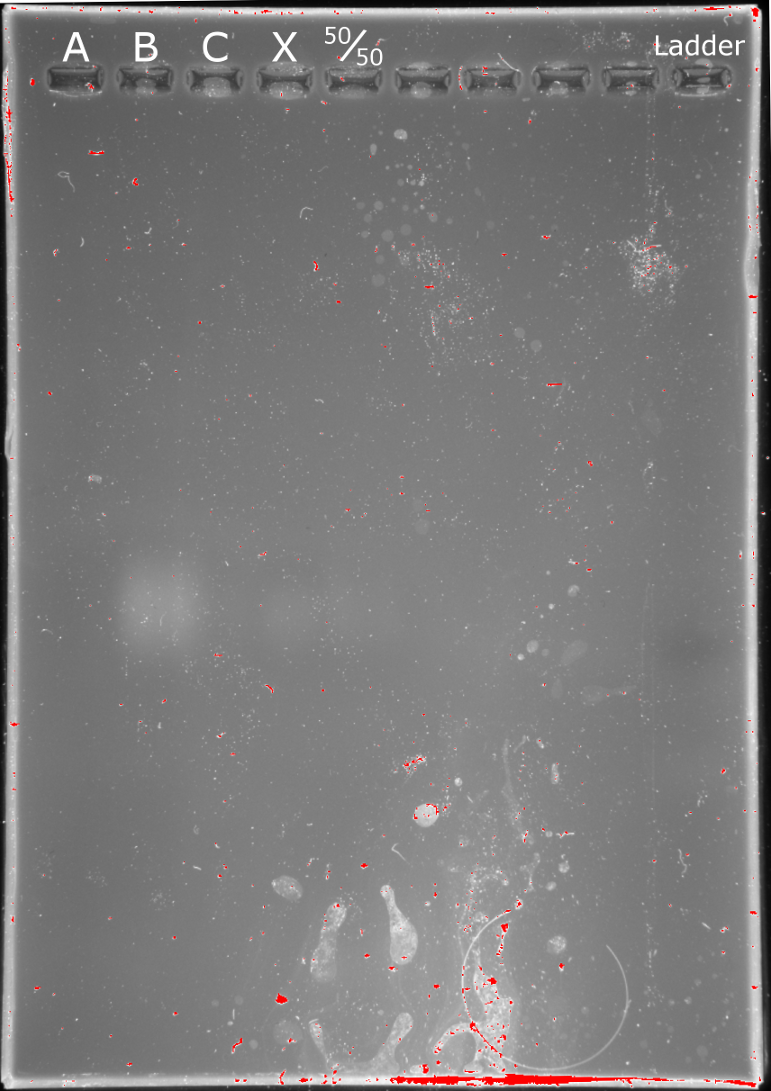
\includegraphics[width=0.3\textwidth]{./gels/view1-stain15min-faintbands-small.png}
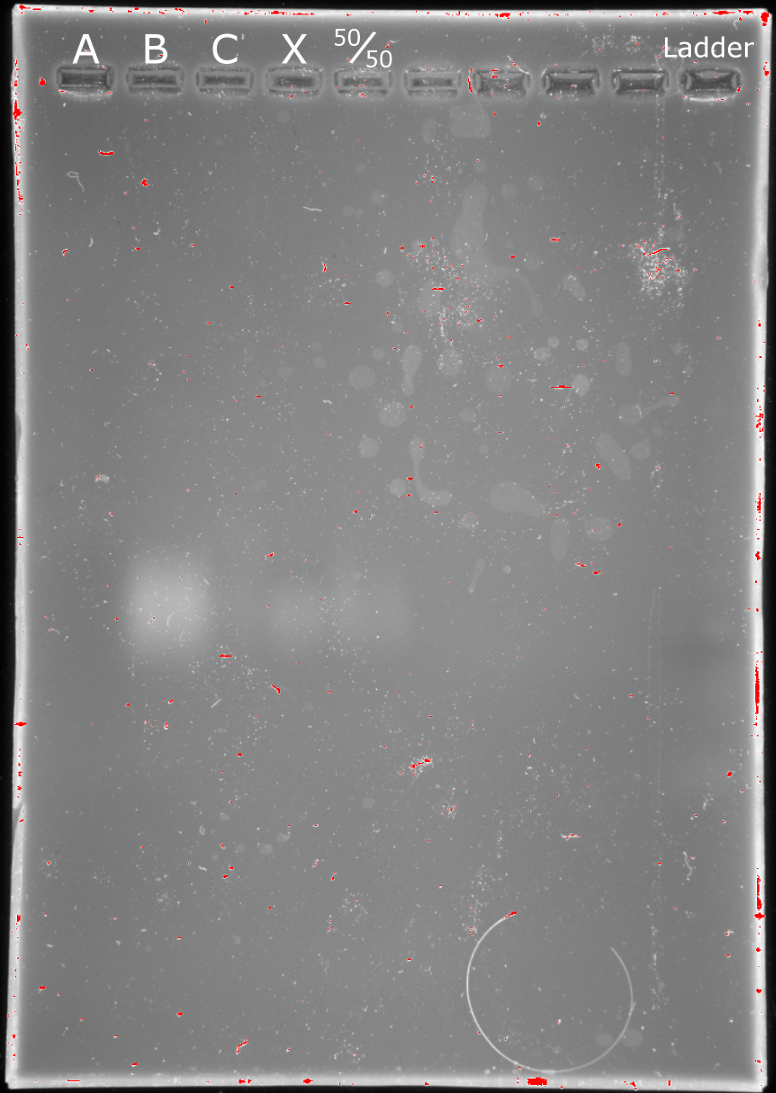
\includegraphics[width=0.3\textwidth]{./gels/view2-stain25min-faintbands-small.png}
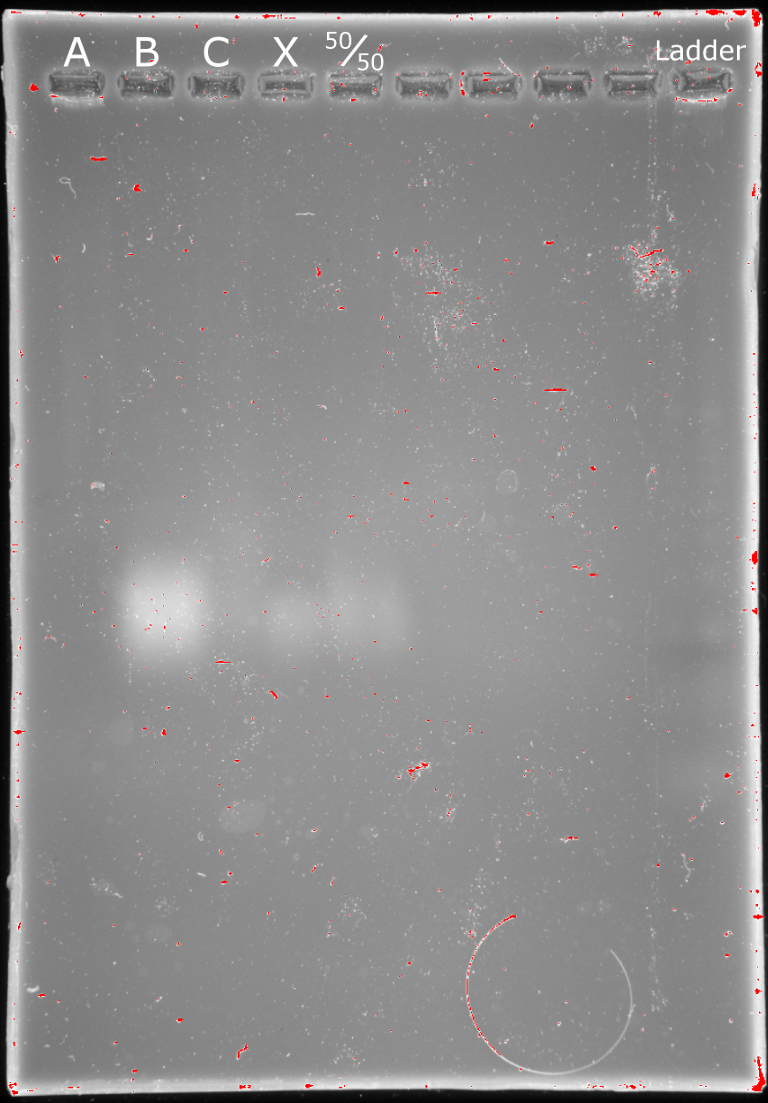
\includegraphics[width=0.3\textwidth]{./gels/view3-stain35min-faintbands-small.png}
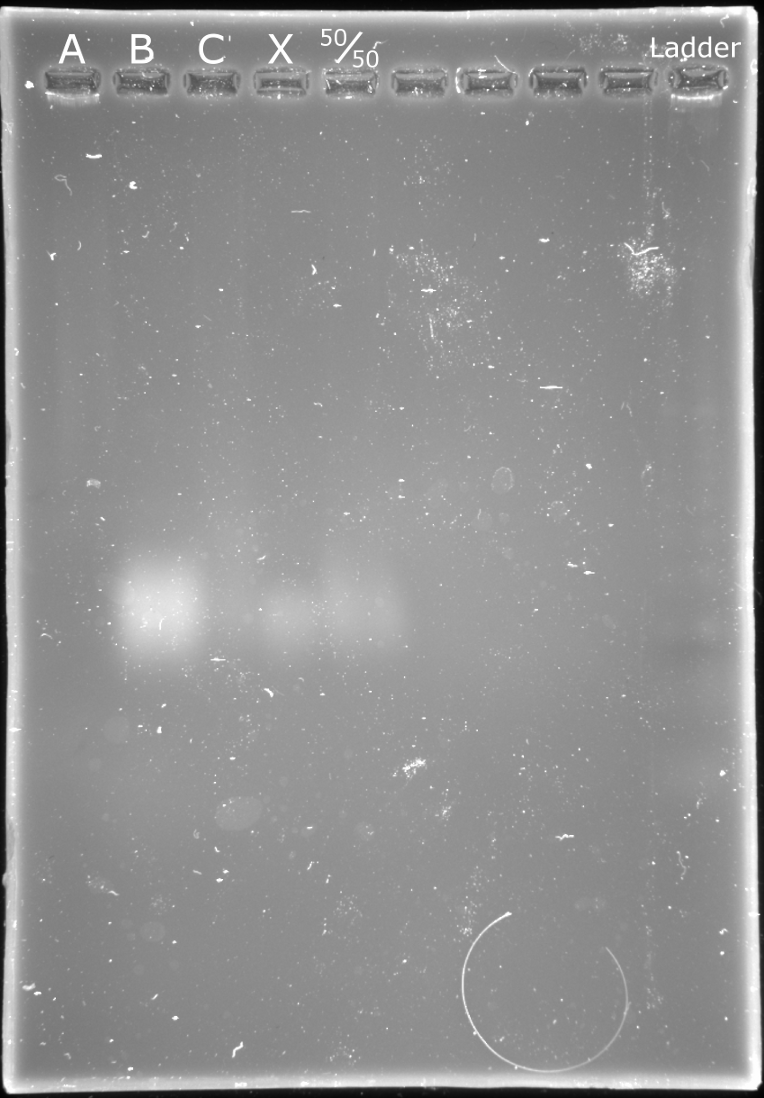
\includegraphics[width=0.3\textwidth]{./gels/view4-stain35min-2secexposure-small.png}
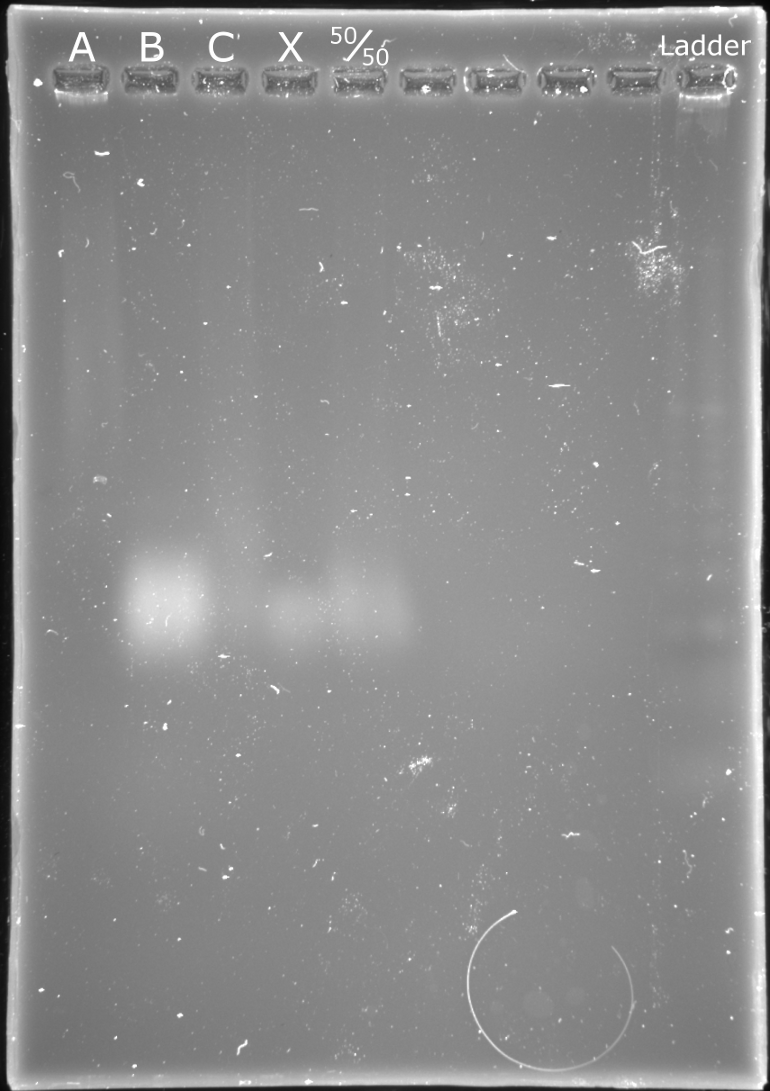
\includegraphics[width=0.3\textwidth]{./gels/view5-stain45min-faintbands-small.png} 
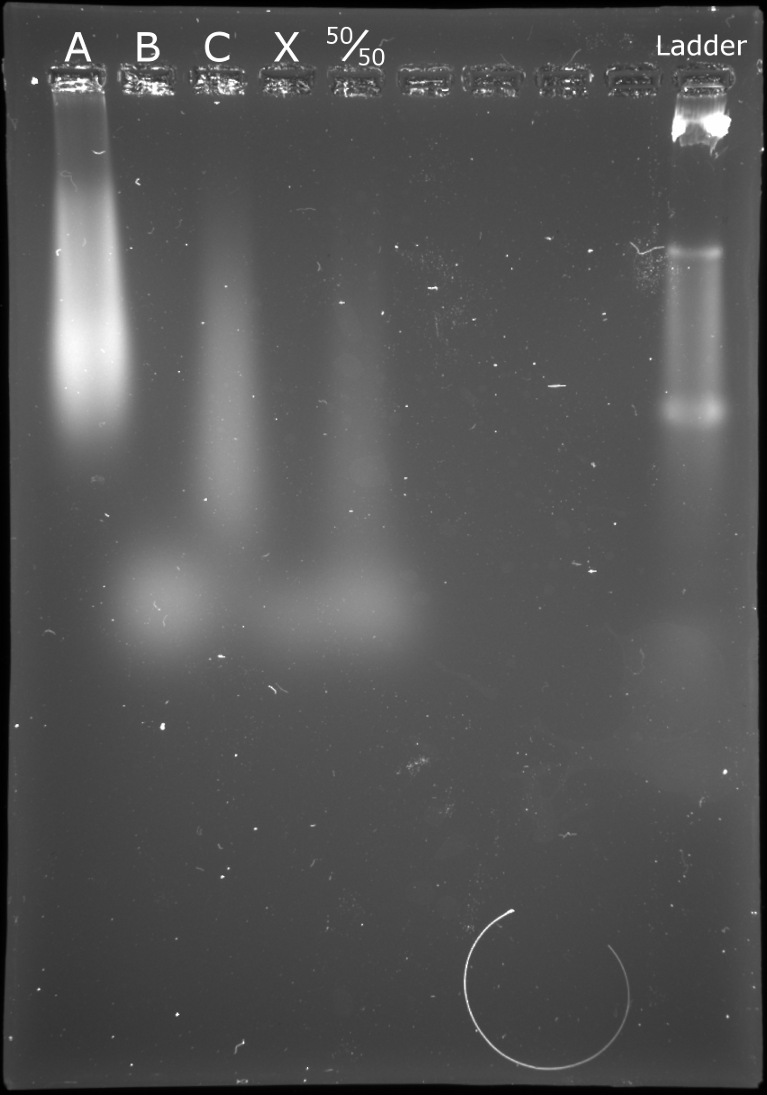
\includegraphics[width=0.3\textwidth]{./gels/view6-stainovernight-faintbands-small.png}
\label{gels}
\caption{From left to right on the top row, we have 15, 25 and 35 minutes of stain with SYBR Gold all exposed for faint bands. On the bottom from left to right, we have a 2 second exposure of the gel after 35 minutes of stain, a faint bands exposure at 45 minutes of stain and finally a faint bands exposure of the gel after it was stained overnight. All staining was preformed with SYBR Gold.}
\end{center}
\end{figure}
\subsection{Procedure Notes}
A 4\% gel was used, where a 2\% gel would have done just as fine. Further, the initial stain should have been 40 minutes, not 15.

\listoffigures
\end{comment}
\bibliographystyle{ieeetr}
\bibliography{biblio}
\end{document}